
% This LaTeX was auto-generated from MATLAB code.
% To make changes, update the MATLAB code and republish this document.

\documentclass{article}
\usepackage[utf8]{inputenc}
\usepackage[spanish]{babel}
\usepackage{amsmath}
\usepackage{amsfonts}
\usepackage{amssymb}
\usepackage{gensymb}
\usepackage{graphicx}
\usepackage{pgfplots}
\usepackage{color}

\sloppy
\definecolor{lightgray}{gray}{0.5}
\setlength{\parindent}{0pt}

\begin{document}

    
    
\subsection*{Contents}

\begin{itemize}
\setlength{\itemsep}{-1ex}
   \item Gr\'aficas
\end{itemize}
\begin{verbatim}
% https://la.mathworks.com/help/symbolic/solve-a-system-of-differential-equations.html
clc;
clear;

syms t vc(t) il(t) C1 C2;

%Valores de los componentes
L=1;
C=1;

%Condiciones Iniciales
v0=1;
i0=0;

%Valores de tiempo y paso
ti=0;
tf=100;
h=0.01;

%Matrices del circuito
%Lleva la forma de:
%M*(dx/dt)+N*x=u(t);

M=[-C 0;0 -L];
N=[0 1;-1 0];
u=[0;0];

%Condiciones iniciales
Xant=[v0;i0];


%Se lleva a la forma
% dx/dt=q(t)-P*x

P=-1.*(M\N)


x=[vc;il];
odes = diff(x) == P*x
constantes = x(0) == Xant;
[vSol(t), iSol(t)] = dsolve(odes,constantes);
vSol(t) = simplify(vSol(t))
iSol(t) = simplify(iSol(t))
\end{verbatim}

        \color{lightgray} \begin{verbatim}
P =

     0     1
    -1     0

 
odes(t) =
 
  diff(vc(t), t) == il(t)
 diff(il(t), t) == -vc(t)
 
 
vSol(t) =
 
-sin(t)
 
 
iSol(t) =
 
cos(t)
 
\end{verbatim} \color{black}
    

\subsection*{Graficas}

\begin{verbatim}
clf
fplot(vSol,[ti,tf])
hold on
fplot(iSol,[ti,tf])
grid on
\end{verbatim}

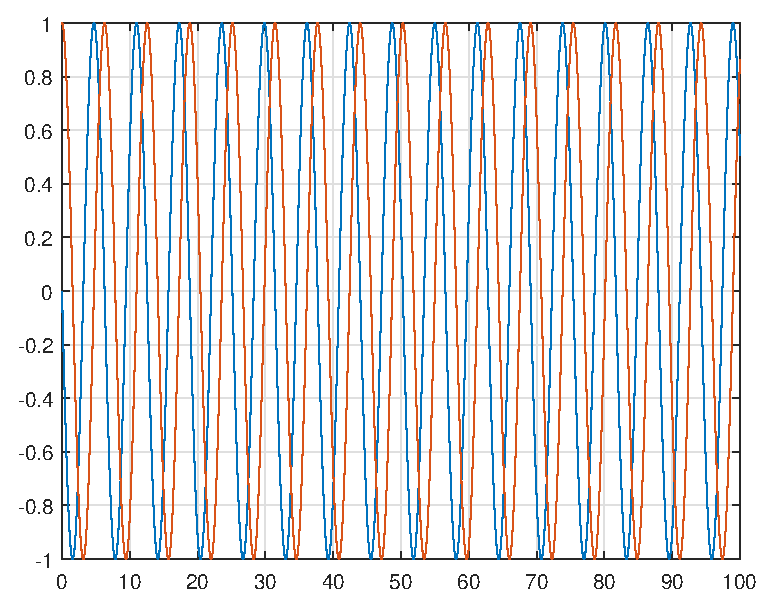
\includegraphics [width=4in]{ejercicio1_01.eps}
\begin{verbatim}
t=ti:h:tf;
v1=eval(subs(vSol));
i1=eval(subs(iSol));

%[T, lambda] = eig(P);
%syms t;
%elambda=diag(exp(eig(P).*t))
%H=T*elambda*inv(T)
%v=H*Xant;
\end{verbatim}



\end{document}
    
